\chapter{Unfallerkennung im Pocket-Mode}




***XYZ***-Nutzern haben die App im Jahr ***XYZ*** installiert und verwendet. Die Anzahl der Motorräder im gleichen Jahr betrugt ***XYZ*** \\ (Quelle: https://de.statista.com/statistik/daten/studie/199228/umfrage/bestand-an-kraftraedern-in-deutschland/). \\

Um die Anzahl der App-Nutzer zu erhöhen wurde eine Umfrage an den damaligen Benutzer der App durchgeführt, um die weitere Bedürfnisse mit weitere bzw. bessere Features abzudecken.

Die zwei wichtigsten Fragen waren:
\begin{itemize}
	\item Wofür nutzen Sie Ihr Smartphone während einer Fahrt mit dem Motorrad?
	\item Wo befindet sich aktuell Ihr Smartphone während der Fahrt normalerweise?
\end{itemize}

In der \autoref{fig:CalimotoUmfragePocketMode} ist das Ergebnis der Umfrage dargestellt. Fast 50\% der befragten nutzen kein Smartphone während einer Fahrt, weil die Strecke bekannt ist oder weil sie Ihre Smartphones nicht am Lenker befestigen wollen. 70\% der Befragten haben Ihre Handys nicht am Motorrad oder am Lenker gehabt sondern in der Tasche bzw. im Rucksack. 
%- Grund: viele fahren nur kurze oder bekannte Strecken und wollen Ihre Handy nicht am Lenker befestigen (oder haben die Möglichkeit nicht). 

%(Figure von der Umfrage Calimoto). ->> Unfallerkennung laufen lassen, auch wenn das Handy in der Tasche ist.\\

%\autoref{fig:CalimotoUmfragePocketMode} zeigt die Daten...

\begin{figure}[H]
	\centering
	\includegraphics[width=\linewidth]{Bilder/CalimotoUmfragePocketMode.png}
	\caption{Calimoto - Umfrage - Pocketmode}
	\label{fig:CalimotoUmfragePocketMode}
\end{figure}

Aus diesem Grund ist die Entwicklung einer Unfallerkennung im Pocket-Mode wichtig, wo das Smartphone nicht mehr unbedingt am Lenker befestigt werden muss. Die Weiterentwicklung der Unfallerkennung wurde mit agilen Methoden erfolgt, \autopageref{abs:MethodenderSoftwareentwicklung}.

\section{Kritische Unfallszenarien}
In \autoref{abs:Unfallerkennungsalgorithmus} wurden der Ablauf der aktuellen Unfallerkennungsalgorithmus sowie deren Parameter (z.B. TipOver) erläutert. Die Entwicklung des Pocket-Modes sollte auf keinen Fall zu Konflikten mit dem normalen Mode führen. Die aktuelle Zuverlässigkeit des Algorithmus' darf durch das Pocket-Mode nicht verringert werden, in dem ein im normalen Mode gut erkennbares Unfallszenario durch das Pocket-Mode übersehen wird.
Um die Konflikte zu vermeiden wird eine Liste der Use- sowie Edgecases vorbereitet, in der die Erwarteten Reaktion des aktuellen Algorithmus' aufgelistet wird. Dadurch erfolgt eine Übersicht der möglichen Konflikten sowie der Fällen, wo ein falscher Alarm ausgelöst werden könnte, und gleich eine mögliche Gegenmaßnahme.



Liste der Edge- und usecases mit einer Erklärung, warum diese kritisch sind und einen Vorschlag, was man dagegen tun kann.
Die \autoref{fig:EdgeCasesExcel} zeigt die erwähnte Liste. Da das Verhalten des Smartphones in der Hosentaschen (am Bein) und am Oberkörper unterschiedlich ist, wurden diese separat betrachtet. In der Spalte 'Beschreibung' ist eine nähere Erklärung des Szenarios erläutert. Die Spalte 'Erkennung durch den Algo' berichtet, ob der aktuelle Algorithmus das Szenario richtig erkennen wird (IO: In Ordnung, NIO: Nicht In Ordnung). Unter 'Bemerkungen' ist eine weitere Erklärung des erwarteten Ergebnisses beschrieben. Bei den kritischen Szenarien, wo der Algorithmus den Fall nicht richtig erkennen würde, wurde eine mögliche Gegenmaßnahme zum Korrigieren der Entscheidung des Algorithmus aufgeschrieben.

\begin{figure}[H]
	\centering
	\includegraphics[width=\linewidth]{Bilder/EdgeCasesExcel.png}
	\caption{Liste der Use- und Edgecases mit der erwarteten Reaktion des Algorithmus'}
	\label{fig:EdgeCasesExcel}
\end{figure}

Nach der internen Statistik ist das Laufen ein häufiger Grund von den falschen Alarmen, deswegen eine Lauferkennung zur Verbesserung der Zuverlässigkeit wichtig.

\section{Lauferkennung} \label{sec:Lauferkennung}
In der bereits bestehenden Version des Algorithmus' ist davon ausgegangen, dass das Smartphone am Lenker befestigt wird. Wenn die Person das Handy nach einer Fahrt in die Hosen- bzw. Jackentasche einsteckt und fängt an zu laufen, wird öfters einen falschen Alarm (falsch-positiv) ausgelöst, da das Laufen im bisherigen Algorithmus nicht berücksichtigt wurde.
Wenn die Unfallerkennung im Pocket-Mode verwendet wird, ist stark zu erwarten, dass die Person nach einer Fahrt oder während einer Pause (z.B. Tanken) vergisst (oder ignoriert), die Unfallerkennung zu deaktivieren, und mit dem Smartphone an sich läuft. Das führt dazu, dass die Anzahl der falschen Alarmen im Pocket-Mode wesentlich steigt.

Um diese falsche Auslösungen zu verhindern, ist eine Lauferkennung wichtig. Diese Arbeit beschäftigt sich im Teil mit der Implementierung der Lauferkennung. Das Ziel dahinter ist das Laufen zu erkennen und die Unfallerkennung temporär zu deaktivieren, um die falsche Alarme zu vermeiden und die Agenten zu entlasten.
In diesem Kapital werden die Schritte der Entwicklung der Lauferkennung erläutert.

% Generated using matlabfrag
% Version: v0.6.16
% Version Date: 04-Apr-2010
% Author: Zebb Prime
%
%% <text>
%
\providecommand\matlabtextA{\color[rgb]{0.150,0.150,0.150}\fontsize{11}{11}\selectfont\strut}%
\psfrag{009}[tc][tc]{\matlabtextA Time (seconds)}%
%
%% </text>
%
%% <xtick>
%
\def\matlabfragNegXTick{\mathord{\makebox[0pt][r]{$-$}}}
%
\providecommand\matlabtextB{\color[rgb]{0.150,0.150,0.150}\fontsize{10}{10}\selectfont\strut}%
\psfrag{000}[ct][ct]{\matlabtextB $405$}%
\psfrag{001}[ct][ct]{\matlabtextB $410$}%
\psfrag{002}[ct][ct]{\matlabtextB $415$}%
\psfrag{003}[ct][ct]{\matlabtextB $420$}%
%
%% </xtick>
%
%% <ytick>
%
\psfrag{004}[rc][rc]{\matlabtextB $-2500$}%
\psfrag{005}[rc][rc]{\matlabtextB $-2000$}%
\psfrag{006}[rc][rc]{\matlabtextB $-1500$}%
\psfrag{007}[rc][rc]{\matlabtextB $-1000$}%
\psfrag{008}[rc][rc]{\matlabtextB $-500$}%
%
%% </ytick>
\begin{figure}[H]
	\centering
	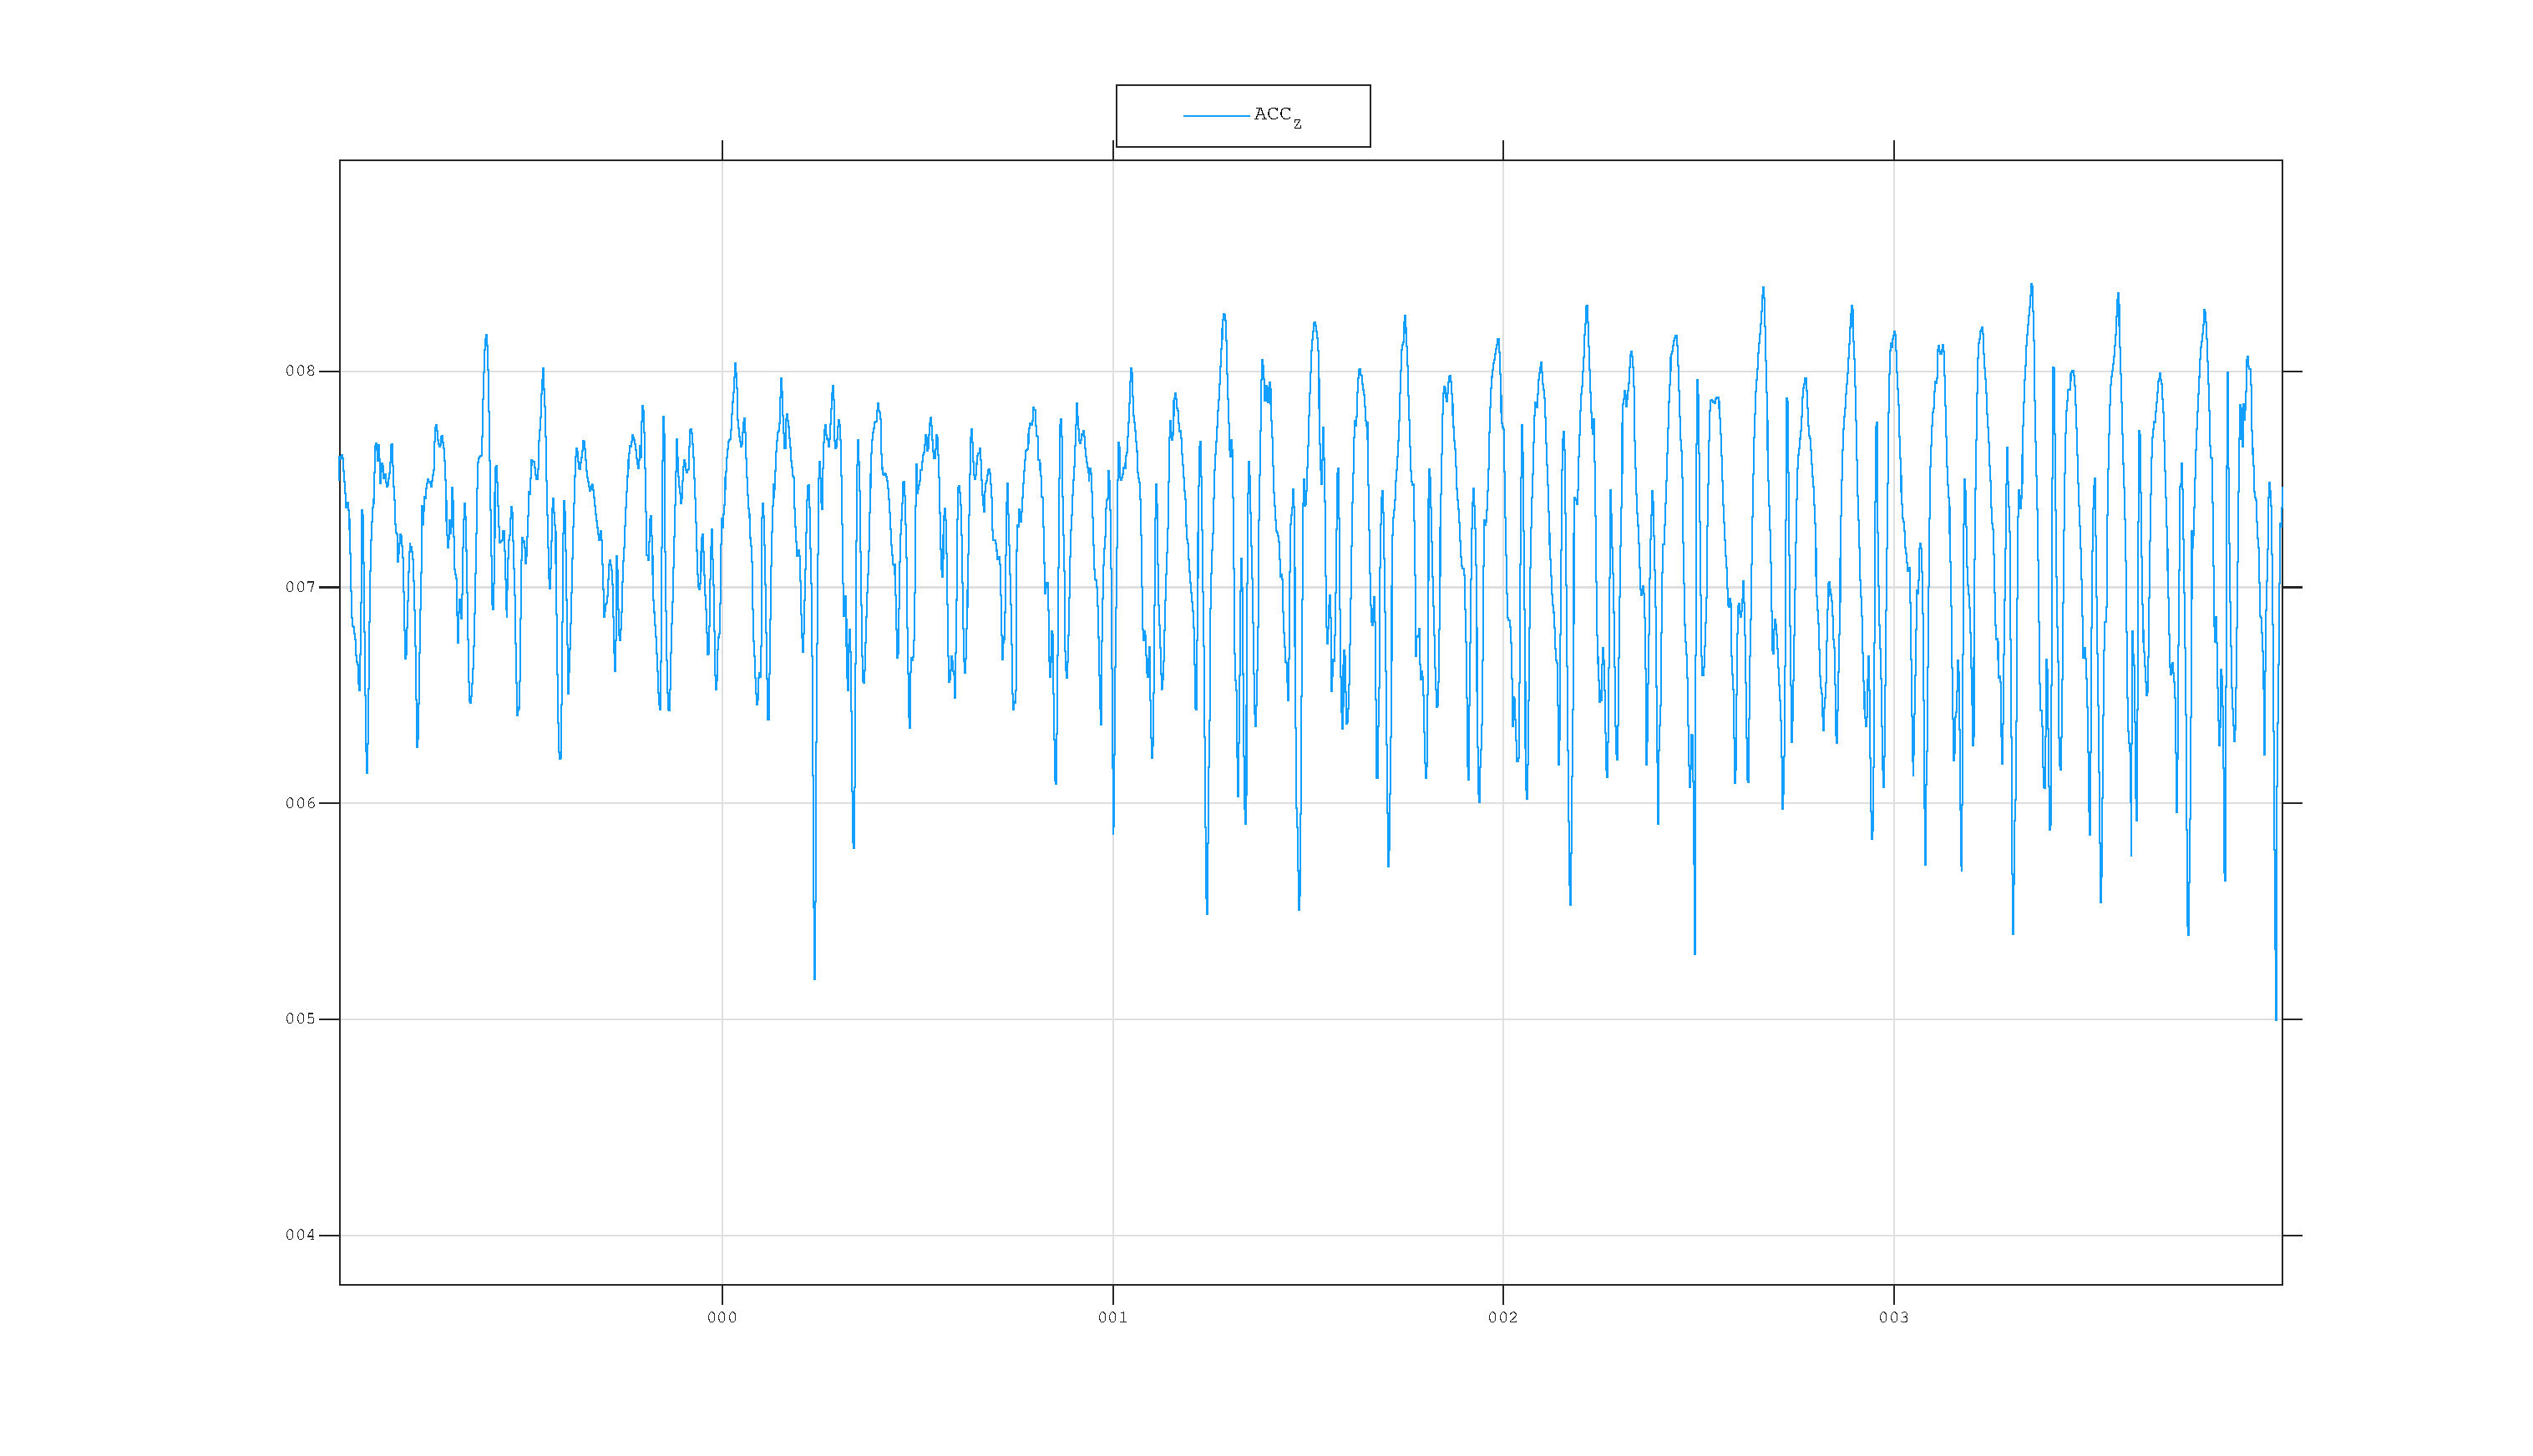
\includegraphics[width=\linewidth]{Bilder/LaufenMuster.eps}
	\caption{Beispiel: Beschleunigungssignal beim Laufen (***x-Achse 0-25 Sekunden, y-Achse (-2500 - 0))}
	\label{fig:LaufenMuster}
\end{figure}
In der \autoref{fig:LaufenMuster} ist ein Beispielsignal aus dem Beschleunigungssensor im Smartphone während des Laufens. Die Person kann bis zu 2 Schritte pro Sekunde im Schnitt zurücklegen. In der Grafik können die Peaks innerhalb einer Sekunde aufgezählt werden und die Anzahl der Schritte ermitteln. Wenn diese unter 2 pro Sekunde sind, ist vom Laufen auszugehen, da ein Motor so wenige Umdrehungen pro Sekunde nicht schafft. Im nächsten Abschnitt werden diese Peaks aufgezählt, um die Anzahl der Schritte bzw. Umdrehungen zu ermitteln.
%
\subsection{1. Idee: Peaks aufzählen} %TODO: ausführlich beschreiben

Wie bereits erwähnt wurde, kann die Person bis zu zwei Schritte pro Sekunde laufen. D.h. aus einem typischen Laufsignal (z.B. \autoref{fig:LaufenMuster}) soll maximal 4 Schritte pro Sekunde aufgezählt werden.
Es soll ein Modell implementiert werden, das die Anzahl der Schritten bzw. der Peaks aufzählt und der Mittelwert davon pro Sekunde zurückgibt. Zur Vereinfachung der Implementierung wurde eine Testumgebung (siehe. \autoref{fig:Lauferkennung_Peaks_Testbeispiel}) aufgebaut. In der Umgebung wurde ein bekanntes Sinussignal generiert und dargestellt.
\begin{figure}[H]
	\centering
	\includegraphics[width=\linewidth]{Bilder/Lauferkennung_Peaks_Testbeispiel.png}
	\caption{Testbeispiel - Lauferkennung - Peaks Zähler}
	\label{fig:Lauferkennung_Peaks_Testbeispiel}
\end{figure}

Die \autoref{fig:Lauferkennung_Peaks_SinusSignalGenerator} zeigt die Spezifikationen des generierten Signals und die \autoref{fig:Lauferkennung_Peaks_SinusSignal} stellt mithilfe eines Scopes (Simulink-Block) das entsprechende Signal grafisch dar sowie wie of das Signal die Nulllinie überschneidet (blau). Aus der Grafik ist die Anzahl der Peaks einfach zu ermitteln und diese beträgt in diesem Fall 100 Hz umgerechnet.
Eine zeitliche Frequenz wird folgendes berechnet:\\
$Freq(Hz) = Freq(rad/sec) / (2 * pi)$; $pi = 3,14$
\begin{figure}[H]
	\centering
	\includegraphics[width=\linewidth]{Bilder/Lauferkennung_Peaks_SinusSignalGenerator.png}
	\caption{Testbeispiel - Lauferkennung - Sinussignalgenerator - Spezifikationen}
	\label{fig:Lauferkennung_Peaks_SinusSignalGenerator}
\end{figure}
\begin{figure}[H]
	\centering
	\includegraphics[width=\linewidth]{Bilder/Lauferkennung_Peaks_SinusSignal.png}
	\caption{Testbeispiel - Lauferkennung - Sinussignal}
	\label{fig:Lauferkennung_Peaks_SinusSignal}
\end{figure}
In dem Modell ist die Funktion 'Zero Crossing' verwendet. Diese zählt wie oft das Signal die x-Achse überquert. Diese Methode liefert das richtige erwartete Ergebnis, wenn das Signal um die x-Achse dargestellt ist. Von der anderen Seite hilft diese Funktion nicht mehr, wenn das Signal eine Offset hat, in dem dieses z.B. um die Linie (y = 300), da in diesem Fall und amplitudenabhängig das Signal die x-Achse nicht mehr schneidet. Das führt dazu, dass das Ergebnis nicht mehr zuverlässig ist.

Eine andere Methode hat sich ergeben, dass die Funktion 'Counter up' in dem Modell verwendet wird. Dieses Block zählt wie oft das Signals in die positive Richtung zeigt. Das neue Implementierung hat ein zuverlässiges Ergebnis im Vergleich zum originalen Modell geliefert.

Beim Einsetzen des gleichen Vorgehens bzw. Modell auf das richtige Laufsignal (\autoref{fig:LaufenMuster}) wurde eine Frequenz von ca. $11$ Hz beim Laufen zurückgegeben.

Nach weiteren Auswertungen und Forschungen wurde der Grund des Fehlers entdeckt. Es lag an den Unterschied zwischen dem perfekten generierten Sinussignal und dem echten Laufsignal. Das echte Signal hat im Vergleich zum generierten viele Störungen (Rauschen). Diese konnten durch das benannte Modell nicht ausgefiltert oder ignoriert werden, was zu einem falschen Ergebnis geführt hat.

%Einen Zähler zu implementieren. Das soll alle Peaks aufzählen mit der Hoffnung, dass es Unterschied zwischen Laufen und Fahren zu erkennen ist.
%Das LaufFrequenz ist zwischen 0.5-4 Hz. Das Fahren ist über 20 Hz.
%Es wurde einen Testbeispiel mit einem Sinussignal gebaut und das Prinzip getestet.


%In der \autoref{fig:Lauferkennung_Peaks_Testbeispiel} ist das Beispielmodell zur Lauferkennung basiert auf das Zählen jedes Peak des Signals. Im Modell wurde ein Sinussignal generiert (\autoref{fig:Lauferkennung_Peaks_SinusSignalGenerator}) und dieses bearbeitet und das Prinzip dadurch getestet.

%\autoref{fig:Lauferkennung_Peaks_SinusSignal} zeigt die Ausgabe der Scope-Funktion. In der Grafik ist das generierte Sinussignal (gelb) sowie wie of das Signal die Nulllinie überschneidet (blau).
%In der Scope-Darstellung sind das originale Sinussignal und ein Zähler sichtbar. Der Zähler hat jeden ‚Zero-crossing‘ aufgezählt.
%Das Testmodell hat die richtige (erwartete) Ergebnisse geliefert: 100 Hz als Frequenz.
%Beim Einsetzen des gleichen Vorgehens auf das richtige Signal ($AccBfX_mg$) (das kalibrierten Signal) wurde eine Frequenz von ca. $11$ Hz beim Laufen und eine Frequenz zwischen $20-30$ Hz ausgerechnet. Das hat die Erwartungen nicht entsprochen.
%Daraus kann folgendes extrahiert werden:
%Beide Signale (Szenarien) (Laufen und Fahren) haben die gleiche Menge von Störungen (Rauschen). Der Unterschied ist die Amplitude. Es kann keine Amplitude ‚Hartkodiert‘ entdeckt werden, da die Amplitude sich ständig ändern kann.
%************ Grafiken von den zwei Signalen darstellen und die Art der Rauschen näher analysieren (was könnte die Ursache sein?); Welche mögliche Lösungen gäbe es dafür? *************\\

%\textbf{Ergebnis: Die Frequenz muss allerdings doch gesucht und schließlich verglichen werden}




\subsection{Frequenzbasierend} %TODO: ausführlich beschreiben

Da die Peakszähler nicht zuverlässig funktioniert hat, war eine bessere Idee notwendig. Das Modell muss die Frequenz des Signal ermitteln und diese denn auswerten.

Dafür ist die FFT ein wichtiges Wort bei einer Frequenzermittlung.

Die App schreibt Messdaten mit der Frequenz von 100 Hz. D.h. pro Sekunde gibt's 100 Messwerte.


Auf die FFT beziehen.\\

zum Berechnen der Frequenz: FFT (Fast Fourier Transformation)\\

Nochmal das gleiche mit dem Testmodel durchgeführt.\\


\begin{figure}[H]
	\centering
	\includegraphics[width=\linewidth]{Bilder/Lauferkennung_Freqbasiert_TestBeispiel_SinussignalGenerator.png}
	\caption{Testbeispiel - Frequenzbasierte Lauferkennung - Sinussignal}
	\label{fig:Lauferkennung_Freqbasiert_TestBeispiel_SinussignalGenerator}
\end{figure}

\begin{figure}[H]
	\centering
	\includegraphics[width=\linewidth]{Bilder/Lauferkennung_Freqbasiert_SpektrumAnalyzerAusgabe.png}
	\caption{Testbeispiel - Frequenzbasierte Lauferkennung - Ausgabe des Spektrum-Analyzer und seine Spezifikationen}
	\label{fig:Lauferkennung_Freqbasiert_SpektrumAnalyzerAusgabe}
\end{figure}

\begin{figure}[H]
	\centering
	\includegraphics[width=\linewidth]{Bilder/Lauferkennung_Freqbasiert_SpektrumAnalyzerAusgabe_gezoomt.png}
	\caption{Testbeispiel - Frequenzbasierte Lauferkennung - Ausgabe des Spektrum-Analyzer im Bereich zwischen 0-0.5 kHz}
	\label{fig:Lauferkennung_Freqbasiert_SpektrumAnalyzerAusgabe_gezoomt}
\end{figure}

\autoref{fig:Lauferkennung_Freqbasiert_SpektrumAnalyzerAusgabe_gezoomt} Es ist schön zu bemerken, dass die Frequenz (100 Hz) sehr gut sichtbar ist. Der obere Teil zeigt die Häufigkeit einer Frequenz (Spektrum) unabhängig von der Zeit. Der untere Teil zeigt die Häufigkeit einer Frequenz mit der Zeit (Spektrogramm).

\begin{figure}[H]
	\centering
	\includegraphics[width=\linewidth]{Bilder/Lauferkennung_Freqbasiert_SpektrumAnalyzerAusgabe_2Einstellungen.png}
	\caption{Testbeispiel - Frequenzbasierte Lauferkennung - Ausgabe des Spektrum-Analyzer mit anderen Spezifikationen}
	\label{fig:Lauferkennung_Freqbasiert_SpektrumAnalyzerAusgabe_2Einstellungen}
\end{figure}

\begin{figure}[H]
	\centering
	\includegraphics[width=\linewidth]{Bilder/Lauferkennung_Freqbasiert_FFT.png}
	\caption{Testbeispiel - Frequenzbasierte Lauferkennung - FFT - Modell}
	\label{fig:Lauferkennung_Freqbasiert_FFT}
\end{figure}

Die AccBfX, AccBfY und AccBfZ sind die Ausgänge des Modells $CalibrationsMotorbike_V2$ und sie sind die Kalibrierte Signale.
Diese Werte werden für die Berechnung der Betrag mit der Formel (**********************)
%TODO: $AccBf_All=√(〖AccBfX〗^2+ 〖AccBfY〗^2+〖AccBfZ〗^2 )$ 
verwendet (\autoref{fig:Lauferkennung_Freqbasiert_FFT}- Nummer 2). Das Ziel ist die Frequenzermittlung richtungsunabhängig zu stellen.
Danach wurde eine FFT an der Variablen $AccBf_All$ durchgeführt, um die Frequenzen zu ermitteln (\autoref{fig:Lauferkennung_Freqbasiert_FFT}- Nummer 2).


\begin{figure}[H]
	\centering
	\includegraphics[width=\linewidth]{Bilder/Lauferkennung_Freqbasiert_FFT_Spezifikationen.png}
	\caption{Testbeispiel - Frequenzbasierte Lauferkennung - FFT - Modell}
	\label{fig:Lauferkennung_Freqbasiert_FFT_Spezifikationen}
\end{figure}
In der \autoref{fig:Lauferkennung_Freqbasiert_FFT_Spezifikationen} wird eine FFT durchgeführt. Die Einstellparameter jedes Element ist ersichtlich.

1-	In der Buffer sind 256 Samples zu betrachten (d.h. ca. 2,5 Sekunden des Signals, da die Abtastrate der Sensor 100 Hz ist). Eine Überlappung von ca. 1 Sekunde wurde auch eingestellt, damit die Zwischen Frequenzen nicht übersehen werden.\\
2-	Der FFT-Typ ist eine Radix-2.\\
3-	Die Ausgabenwerte der FFT durch 265 dividieren. (warum?)\\ %TODO: warum 
4-	Betrag des FFT-Ausgangs bilden (warum?)\\ %TODO: warum 
5-	Da FFT ein gespiegelter Ausgang liefert wird nur die Hälfte der Matrix angenommen (1:128)\\
\subsubsection{Entscheidungskriterien - Matlabskript}
%
%
%
%
%
Screenshot vom Skript mit einer Erklärung (\autoref{fig:MatlabSkript}) %TODO: Skript erklären und eine Ablaufschema (Entscheidungsbaum) erstellen
\begin{figure}[H]
	\centering
	\includegraphics[width=\linewidth]{Bilder/MatlabSkript.png}
	\caption{Entscheidungsskript durch mehrere Kriterien (Frequenz und Geschwindigkeit)}
	\label{fig:MatlabSkript}
\end{figure}




\subsubsection{Beispiel}
Mögliche Konflikte: ID = 2488; CrashNoPSAP;\\

\begin{figure}[H]
	\centering
	\includegraphics[width=\linewidth]{Bilder/Lauferkennung_Freqbasiert_Ausgangsbeispiel.png}
	\caption{Testbeispiel - Frequenzbasierte Lauferkennung - Ausgangsbeispiel - ID 2488}
	\label{fig:Lauferkennung_Freqbasiert_Ausgangsbeispiel_ID2488}
\end{figure}
Da hier (\autoref{fig:Lauferkennung_Freqbasiert_Ausgangsbeispiel_ID2488} und \autoref{fig:Lauferkennung_Freqbasiert_Ausgangsbeispiel_ID2488_Scope}) die maximale Intensität der Frequenz 1,5, wird diese als das Maximum übernommen und weiterbearbeitet. Die nächste größte Intensität liegt sehr nah dazu und hat die Frequenz 21,88 Hz, was eigentlich richtiger ist.

\begin{figure}[H]
	\centering
	\includegraphics[width=\linewidth]{Bilder/Lauferkennung_Freqbasiert_Ausgangsbeispiel_ID2488_Scope.png}
	\caption{Testbeispiel - Frequenzbasierte Lauferkennung - Ausgangsbeispiel - ID 2488 - Scope}
	\label{fig:Lauferkennung_Freqbasiert_Ausgangsbeispiel_ID2488_Scope}
\end{figure}




\subsubsection{Werte Sinnvoll auswählen}
- gültige Intensität\\
- Frequenzbereiche\\
- Gültige Geschwindigkeit\\
- Ausschlusskriterien\\





\section{Verifikation des Algorithmus'}
% Aufgrund der Verifizierung des Algorithmus werden im Folgenden statistische Zahlen über Fahrradunfälle weltweit sowie in Deutschland dargestellt. Danach wird eine statistische Fallzahlabschätzung durchgeführt, um die notwendige Anzahl der Versuche zu ermitteln. Eine Versuchsplannung wird anhand der Ergebnisse der Versuche durchgeführt, die bereits vor der eigentlichen Verifizierung durchgeführt wurden. 
%
%
%


\subsection{Groundtruth sammeln}

- Videos mit den Daten synchronisieren (Das Tool erläutern? oder vllt. nur erwähnen?)\\
- Groundtruth labels nachdenken und erläutern\\
- Videos labeln\\









%\begin{table}\caption{Statistische Zahlen über Unfälle in Deutschland \cite{Verkehrsunfaelle_Fahrrad2017}} 
%	\centering
%	\begin{tabular}{|p{3.2cm}|>{\centering\arraybackslash}p{3.3cm}|>{\centering\arraybackslash}p{3.3cm}|>{\centering\arraybackslash}p{3.3cm}|}
	%		\hline
	%		\textbf{Jahr} & \textbf{Unfälle} & \textbf{Verunglückte} & \textbf{Getötete} \\
	%		\hline
	%		2000 & 382.949 & 511.577 & 7.503 \\
	%		\hline
	%		2005 & 336.619 & 438.804 & 5.361 \\
	%		\hline
	%		2010 & 288.297 & 374.818 & 3.648 \\
	%		\hline
	%		2014 & 302.435 & 392.912 & 3.377 \\
	%		\hline
	%		2015 & 305.659 & 396.891 & 3.459 \\
	%		\hline
	%		2016 & 308.145 & 399.872 & 3.206 \\
	%		\hline
	%		2017 & 302.656 & 393.492 & 3.180 \\
	%		\hline
	%	\end{tabular}
%	\label{tab:UnfallImJahren}
%\end{table}







